\documentclass{article}
\usepackage{tikz}
\usepackage{CJKutf8}
\usepackage{amsmath}
\usepackage{amsthm}
\begin{document}
\begin{CJK}{UTF8}{gbsn}
  \newtheorem*{Exercise}{习题}
  \newtheorem*{Def}{定义}
  \huge
    \begin{Def}
    设$G=(V,E)$, $H = (U, F)$为两个图,如果存在一个一一对应$\phi:V \to
    U$,使得$\{u,v\} \in E$当且仅当$\{\phi(u),\phi(v)\} \in F$,则称$G$与$H$同构。
  \end{Def}
    \begin{minipage}[c]{0.4\textwidth}
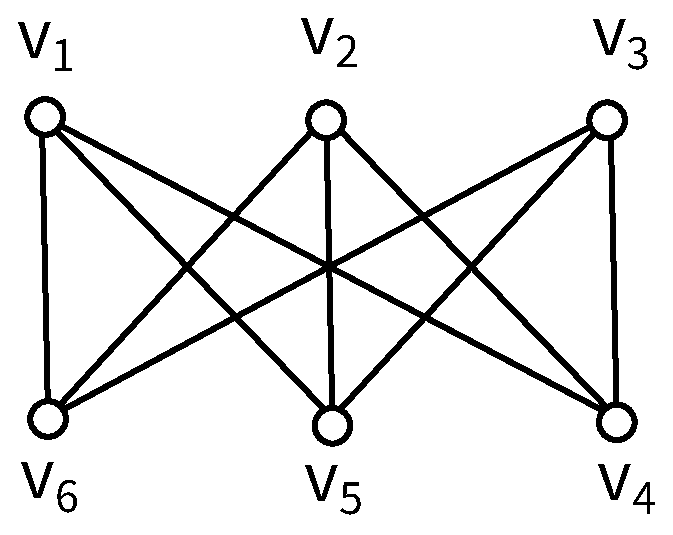
\includegraphics[width=4cm,height=3cm]{k33} \\ \centering G 
    \end{minipage}\hspace{2cm}
    \begin{minipage}[c]{0.4\textwidth}
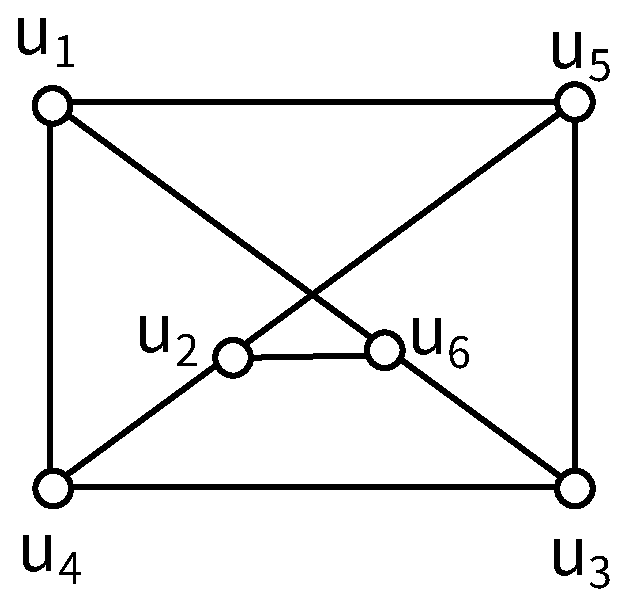
\includegraphics[width=4cm,height=3cm]{isomorphic} \\ \centering H 
    \end{minipage}

\end{CJK}
\end{document}


%%% Local Variables:
%%% mode: latex
%%% TeX-master: t
%%% End:
